%-----------------------------------------------------------------
%	CONCLUSIONS
%	!TEX root = ./../main.tex
%-----------------------------------------------------------------
\section{Results and Discussion}

In \cref{tab:result}, we can see one optimal solution found using our algorithm. The vector $\va{x}$  shows the indicator of item $i$ accepted inside the trucks, for instance since the value $x_1$ is \num{1}, and $x_2$ is \num{0}, hence item 1 is accepted and item 2 is not accepted inside truck. In \cref{tab:result} is also shown the total value that we want to maximize. The result of the maximum value is $f = 598$ with the total weight is exactly $\SI{600}{\kg}$ which is the upper bound or maximum weight $W$ of goods which the truck can carry.

\begin{table}[H]
    \centering
    \begin{tabularx}{0.9\textwidth}{c X}
        \toprule
        \toprule
        Variable & Optimal value \\
        \midrule
        $\va{x}$     & \texttt{[1 0 1 1 1 0 1 1 1 1 1 0 1 1 1 1 1 1 1 1 1 1 0 1 0 1 0 1 1 1 1 1 0 0 1 1 1 1 1 1 1 0 1 1 1 1 1 1 0 1]} \\
        Total Value  & 598 \\
        Total Weight & 600 \\
        \bottomrule
    \end{tabularx}
    \caption{Optimal Solution for the Knapsack Problem}
    \label{tab:result}
\end{table}

Fig.~\ref{fig:values} and \cref{fig:weights} show the evolution of the total value and total weight of the computed, respectively. As it can be seen, the convergence to the optimal solution is quite fast in the initial iterations of the algorithm ($\lesssim \num{200000}$ iterations) and then the slow decreasing of the temperature allows the algorithm to find the optimal combination of items in the solution space. One could say that after iteration \num{400000} the system reaches the freezing point; although this is not a problem, since the solution has already been found.

\begin{figure}[H]
    \centering
    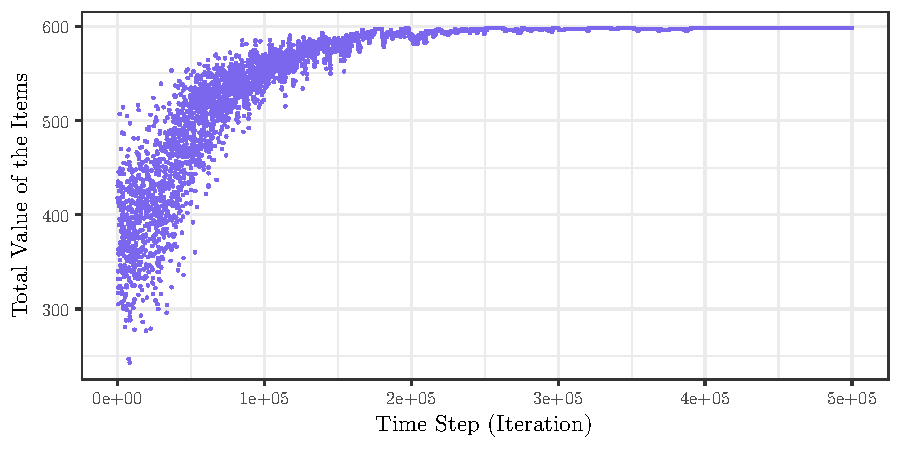
\includegraphics[width=\textwidth]{images/value}
    \caption{Evolution of the Total Value of the Items in the Truck}
    \label{fig:values}
\end{figure}

\begin{figure}[H]
    \centering
    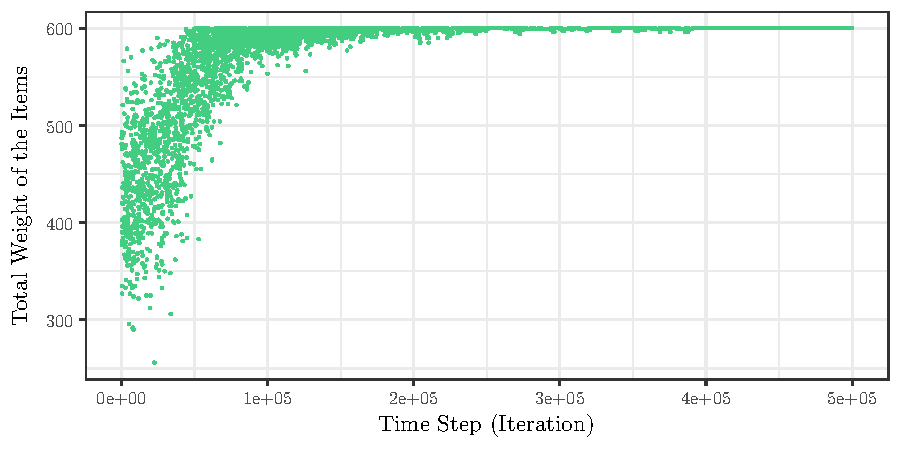
\includegraphics[width=\textwidth]{images/weight}
    \caption{Evolution of the Total Weight of the Items in the Truck}
    \label{fig:weights}
\end{figure}



\subsection*{Future Work}

Some different experiments, for instance tuning the parameters have been left for the future work due to lack of time. There are some ideas that we would like to try during the implementation of simulated annealing algorithm to solve the knapsack problem. This analysis report mainly focused on maximizing the values with only considering only maximum one item of each good allowed in the truck. For this reason, we propose some ideas to be tested and implemented as part of future work and further improvements as follows:
\begin{enumerate}[(i)]
	\item Solving knapsack problems with subjects to more constraints, for instance solving knapsack problem that allows more than one item to put inside the truck. This problem is so-called multidimensional knapsack problem. \cite{Qian2007}
    \item Tune the parameters of the program, such as the Cooling Schedule, and mainly the process of moving in the solution space.
\end{enumerate}